\documentclass[11pt,fleqn]{article}
\usepackage{../cs188,latexsym,epsf, amsmath,amsfonts,graphicx,url,multicol}
\lecture{5}
\def\title{Note \the\lecturenumber}
\begin{document}
\maketitle


\iffalse
\documentclass[11pt,fleqn]{article}
\usepackage{latexsym,epsf,amsmath,amsfonts,graphicx,url}

\title{Note 5}

\newcommand{\F}{\mathbb{F}}
\newcommand{\Z}{\mathbb{Z}}
\newcommand{\Q}{\mathbb{Q}}
\newcommand{\R}{\mathbb{R}}
\newcommand{\C}{\mathbb{C}}

\begin{document}

\maketitle
\fi

\section*{Reinforcement Learning}
In the previous note, we discussed Markov decision processes, which we solved using techniques such as value iteration and policy iteration to compute the optimal values of states and extract optimal policies. Solving Markov decision processes is an example of \textbf{offline planning}, where agents have full knowledge of both the transition function and the reward function, all the knowledge they need to precompute optimal actions in the world encoded by the MDP without ever actually taking any actions. In this note, we'll discuss \textbf{online planning}, during which an agent has no prior knowledge of rewards or transitions in the world (still represented as a MDP). In online planning, an agent first tries \textbf{exploration}, during which it performs actions either randomly or under some policy and receives \textbf{feedback} in the form of the successor states it ends up in and the corresponding rewards it reaps. The agent uses this feedback to predict an optimal policy, a process known as \textbf{reinforcement learning}, before using this predicted policy for \textbf{exploitation}.
\begin{center}	
	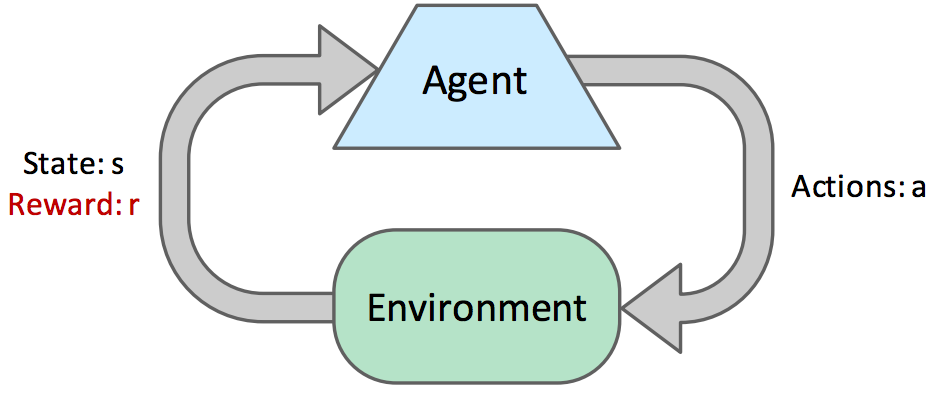
\includegraphics[width=10cm]{img/feedback-loop}
\end{center}
Let's start with some basic terminology. At each timestep during online planning, an agent starts in a state $s$, then takes an action $a$ and ends up in a successor state $s'$, attaining some reward $r$. Each $(s, a, s', r)$ tuple is known as a \textbf{sample}. Often, an agent continues to take actions and collect samples in succession until arriving at a terminal state. Such a string of samples is known as an \textbf{episode}. Agents typically go through many episodes during exploration in order to collect sufficient data needed for learning.

There are two types of reinforcement learning, \textbf{model-based learning} and \textbf{model-free learning}. Model-based learning attempts to estimate the transition and reward functions with the samples attained during exploration before using these estimates to solve the MDP normally with value or policy iteration. Model-free learning, on the other hand, attempts to estimate the q-values of states directly, without ever using any memory to construct a model of the rewards and transitions in the MDP.

\section*{Model-Based Learning}
In model-based learning an agent generates an approximation of the transition function, $\hat{T}(s, a, s')$, by keeping counts of the number of times it arrives in each state $s'$ after entering each q-state $(s, a)$. The agent can then estimate values of $\hat{T}(s, a, s')$ upon request by \textbf{normalizing} the counts it has collected - dividing the count for each tuple $(s, a, s')$ by the sum over all counts where the agent was in q-state $(s, a)$. Normalization of counts allows them to be interpreted as probabilities. Consider the following example MDP with states $S = \{A, B, C, D, E, x\}$, with $x$ representing a terminal state, and discount factor $\gamma = 1$:
	\begin{center}
		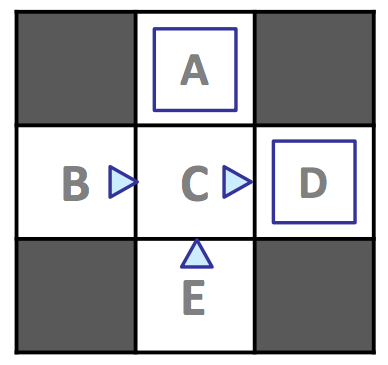
\includegraphics[width=5cm]{img/rl-example-1}
	\end{center}
Assume we allow our agent to explore the MDP for four episodes under the policy $\pi_{explore}$ delineated above (a directional triangle indicates motion in the direction the triangle points, and a blue squares represents taking $exit$ as the action of choice), and yield the following results:
	\begin{center}
		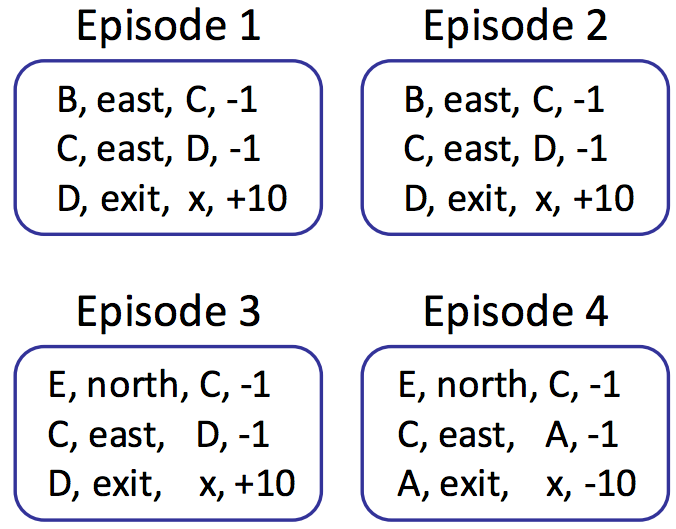
\includegraphics[width=8cm]{img/example-1-episodes}
	\end{center}
We now have a collective $12$ samples, $3$ from each episode with counts as follows:
\begin{center}
\begin{tabular}{ |c|c|c|c| } 
 \hline
 \textbf{s} & \textbf{a} & \textbf{s$'$} & \textbf{count} \\ 
 \hline
 $A$ & $exit$ & $x$ & 1\\
 \hline
 $B$ & $east$ & $C$ & 2\\ 
 \hline
 $C$ & $east$ & $A$ & 1\\
 \hline
 $C$ & $east$ & $D$ & 3\\ 
 \hline
 $D$ & $exit$ & $x$ & 3\\ 
 \hline
 $E$ & $north$ & $C$ & 2\\ 
 \hline
\end{tabular}
\end{center}
Recalling that $T(s, a, s') = P(s' | a, s)$, we can estimate the transition function with these counts by dividing the counts for each tuple $(s, a, s')$ by the total number of times we were in q-state $(s, a)$ and the reward function directly from the rewards we reaped during exploration:
\begin{multicols}{2}
\begin{itemize}
\item{\textbf{Transition Function}: $\:\: \hat{T}(s, a, s')$}
	\begin{itemize}
		\item $\hat{T}(A, exit, x) = \frac{\#(A, exit, x)}{\#(A, exit)} = \frac{1}{1} = 1$
		\item $\hat{T}(B, east, C) = \frac{\#(B, east, C)}{\#(B, east)} = \frac{2}{2} = 1$
		\item $\hat{T}(C, east, A) = \frac{\#(C, east, A)}{\#(C, east)} = \frac{1}{4} = 0.25$
		\item $\hat{T}(C, east, D) = \frac{\#(C, east, D)}{\#(C, east)} = \frac{3}{4} = 0.75$
		\item $\hat{T}(D, exit, x) = \frac{\#(D, exit, x)}{\#(D, exit)} = \frac{3}{3} = 1$
		\item $\hat{T}(E, north, C) = \frac{\#(E, north, C)}{\#(E, north)} = \frac{2}{2} = 1$
	\end{itemize}
\item{\textbf{Reward Function}: $\:\: \hat{R}(s, a, s')$}
	\vspace{-3.2mm}
	\begin{itemize}
		\item $\hat{R}(A, exit, x) = -10$
		\item $\hat{R}(B, east, C) = -1$
		\item $\hat{R}(C, east, A) = -1$
		\item $\hat{R}(C, east, D) = -1$
		\item $\hat{R}(D, exit, x) = +10$
		\item $\hat{R}(E, north, C) = -1$
	\end{itemize}
\end{itemize}
\end{multicols} 
Under the \textbf{law of large numbers}, as we collect more and more samples by having our agent experience more episodes, our models of $\hat{T}$ and $\hat{R}$ will improve, with $\hat{T}$ converging towards $T$ and $\hat{R}$ acquiring knowledge of new rewards as we discover new $(s, a, s')$ tuples. Whenever we see fit, we can end our agent's training to generate a policy $\pi_{exploit}$ by running value or policy iteration with our current models for $\hat{T}$ and $\hat{R}$ and use $\pi_{exploit}$ for exploitation, having our agent traverse the MDP taking actions seeking reward maximization rather than seeking learning. It's common practice to have agents follow $\pi_{explore}$ with some defined probability $p_{explore}$ (and $\pi_{exploit}$ with probability $(1 - p_{explore})$) at any given timestep. Over time, as the agent's model of $\hat{T}$ and $\hat{R}$ improve, $p_{explore}$ is decreased towards 0, and exploitation becomes more and more prevalent over exploration. 

Model-free learning is very effective yet remarkably simple and intuitive, generating $\hat{T}$ and $\hat{R}$ with nothing more than counting and normalization. However, it can be expensive to maintain counts for every $(s, a, s')$ tuple seen and so in the next section on model-free learning, we'll develop methods to bypass maintaining counts altogether and avoid the memory overhead of model-based learning.

\section*{Model-Free Learning}

\end{document}